\chapter{The Roofline Performance Model}\label{v0ch:22}
\begin{chaptersummary}
Having obtained a solution algorithm, we next identify runtime limits. Arithmetic intensity connects throughput with data movement, giving testable Roofline bounds. Later discretizations use the same analysis, provided work, memory level, and timing scope agree. Identify the limiting resource before choosing an optimization.
\end{chaptersummary}
\learninggoals{Count FLOPs and bytes and locate the ridge point; distinguish theoretical peaks, sustained bandwidth, and measured throughput; compare GEMM and SpMV.}
\paragraph{Core Question}Why do floating-point kernels achieve widely different throughput?

\section{Two Resource Bounds}
For work $F$ FLOPs, traffic $Q$ bytes at a specified memory level, sustained bandwidth $B$ bytes/s, and precision-specific peak $P_{\rm peak}$ FLOP/s,
\[
 I=F/Q,\quad P_{\rm attained}=F/T,\qquad
 P_{\rm attained}\le\min(P_{\rm peak},BI),\qquad
 I_{\rm ridge}=P_{\rm peak}/B.
\]
Roofline plots arithmetic intensity against throughput to expose resource bounds.\cite{roofline}
The model organizes performance analysis; computation, storage, and communication limits predate it. Latency, dependencies, instruction mix, insufficient parallelism, and imbalance can place performance below the roof.
Pipelines, vector units, multicore processors, and accelerators increase arithmetic throughput, while memory latency and bandwidth need not improve proportionally: the memory wall. Caches, blocking, and batching mitigate this imbalance through reuse. Machine balance $P_{\rm peak}/B$ sets the intensity needed to become compute-bound.\cite{architecture}
Peak utilization is $P_{\rm attained}/P_{\rm peak}$; Roofline-relative utilization is $P_{\rm attained}/\min(P_{\rm peak},BI)$. Both require consistent precision, work, and traffic definitions and measure different efficiencies.
\conceptbridge{Why is counting additions and multiplications insufficient?}{The same arithmetic may reuse register data or wait for fresh operands. Intensity relates work to movement at a chosen memory level. Reducing FLOPs may leave limiting traffic unchanged, even lowering reported throughput while shortening runtime.}{Operator work $\longrightarrow$ data reuse $\longrightarrow$ limiting resources and runtime.}
\section{GEMM and CSR-SpMV}
Dense square multiplication $C=AB$ costs approximately $2n^3$ FLOPs. Reading each input and writing the output once gives an ideal double-precision $24n^2$ bytes and intensity $n/12$. Cache capacity, blocking, and write allocation alter actual traffic.
CSR-SpMV counts one multiply-add, or 2 FLOPs, per nonzero. Double-precision values and 32-bit column indices require at least 12 bytes, plus row pointers, $\bm x$ access, and output. Intensity generally remains low even with substantial $\bm x$ reuse. Index width, cache hits, and access patterns determine the specific byte model.
\section{Models, Timing, and Calibration}
The schematic uses assumed values $P_{\rm peak}=1000$ GFLOP/s and $B=100$ GB/s, with a ridge at 10 FLOP/byte, to illustrate the roof geometry. CPU kernel plots instead use measured times and work models. Positioning those measurements against local hardware roofs requires a separate calibration.
\begin{figure}[htbp]\centering
\IfFileExists{Vol0_Linear_Algebra_HPC/figures/roofline_model.pdf}{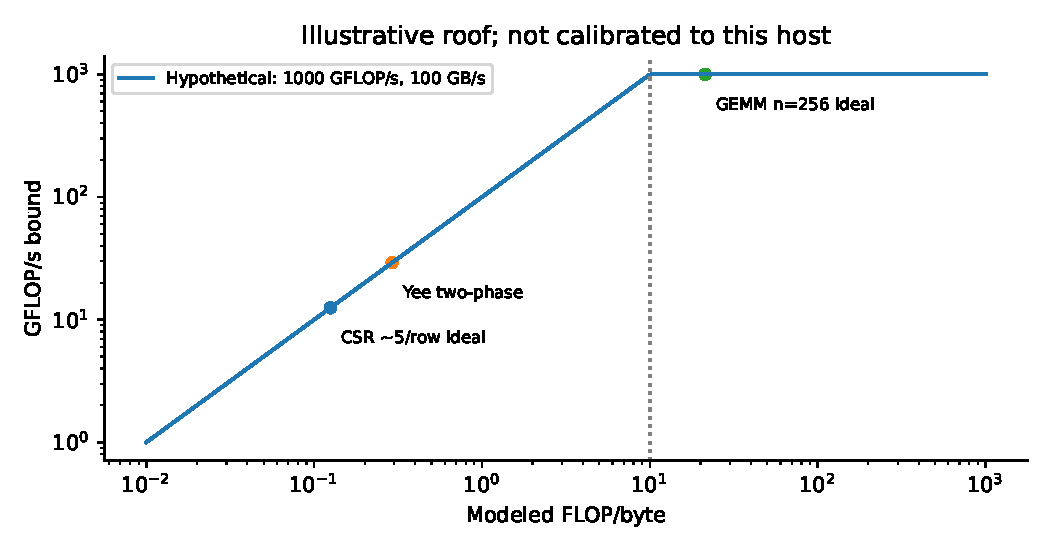
\includegraphics[width=.84\textwidth]{Vol0_Linear_Algebra_HPC/figures/roofline_model.pdf}}{}
\caption{Roofline for hypothetical hardware; neither the roof nor the byte model is a DRAM-counter measurement.}
\end{figure}
Calibration separately measures sustained bandwidth, precision-specific throughput, and actual traffic. Different cache levels can have different roofs. DRAM models do not describe cache-resident small arrays.
\costnote{Bandwidth-bound kernels benefit from reduced traffic, reuse, and layout improvements; compute-bound kernels benefit from vectorization and instruction efficiency. GFLOP/s diagnoses resource use, while total time at fixed error measures computational benefit.}
\coderef{roofline/kernels.py}
\aiexercise{For CSR with 32- and 64-bit indices, derive ideal-reuse and per-nonzero $x$-read traffic models. Compute intensities and identify omitted write-allocation effects.}{Given GEMM/SpMV times and array sizes, determine whether they can share one DRAM Roofline and identify missing measurements.}
\studyroute{Hardware-counter calibration and empirical hierarchical-Roofline tooling are omitted. See \cite{roofline,cuda}.}{arithmetic intensity; operational intensity; ridge point; sustained bandwidth; hierarchical Roofline}
